\section{Ejemplos y ejercicios} \label{ejemplos-ejs}

	\subsection{Ejemplos} \label{ejemplo1}
		\begin{frame}{Ejemplo 1}
			Considérese el ejemplo de problema de valores iniciales dado en la motivación.

			\begin{equation*}
			\begin{cases}
			y'(t) = -4 t^3 y^2 \\
			y(-10) = 1/10001 \\
			t \in [-10,0] \\
			\end{cases}
			\end{equation*}

			cuando se resuelve mediante el método de Euler y con el método del Trapecio Explícito e Iterativo, con paso $10^{-3}$. se obtienen la siguiente gráfica. El método del Trapecio Iterativo usa una tolerancia de $10^{-4}$.
		\end{frame}


		\begin{frame}{Ejemplo 1}	
			\begin{figure}[h]
				\centering
				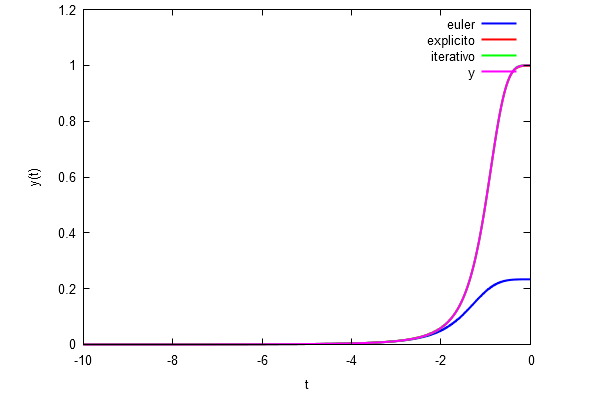
\includegraphics[width=10cm]{./Images/ej1.png}
				\caption{Aproximación a la solución con los distintos métodos.}
			\end{figure}
		\end{frame}	
		
		
		\begin{frame}{Ejemplo 2}
			Considérese el problema de valores iniciales
			
			\begin{equation*}
			\begin{cases}
			y'(t) = -1 + \frac{y}{t} \\
			y(1) = 0
			\end{cases}
			\end{equation*}
			
			calcular el valor de $y(2)$ para $h=0.25$ y $h=0.1$.			
		\end{frame}
		
		\begin{frame}{Ejemplo 2}
			\begin{table}[H]
				\centering
				\begin{tabular}{|| c | c | c | c | c ||}
					\hline
					\hline $j$ &  $t_{j-1}$ & $y_{j-1}$ & $t_j$ & $y_j$ \\
					\hline 1 & 1.00 & 0.000000 & 1.25 & -0.275000 \\
					\hline 2 & 1.05 & -0.275000 & 1.50 & -0.600833 \\
					\hline 3 & 1.10 & -0.600833 & 1.75 & -0.968829 \\
					\hline 4 & 1.15 & -0.968829 & 2.00 & -1.372859 \\
					\hline
					\hline
				\end{tabular}
				\caption{Trapecio con $h=0.25$}
				\label{table:trapecio-ejemplo2.1}
			\end{table}		
		\end{frame}
		
		\begin{frame}{Ejemplo 2}
				\begin{table}[H]
					\centering
					\begin{tabular}{|| c | c | c | c | c ||}
						\hline
						\hline $j$ &  $t_{j-1}$ & $y_{j-1}$ & $t_j$ & $y_j$ \\
						\hline 1 & 0.00 & 0.000000 & 0.10 & -0.104545 \\
						\hline 2 & 0.10 & -0.104545 & 0.20 & -0.218216 \\
						\hline 3 & 0.20 & -0.218216 & 0.20 & -0.340247 \\
						\hline 4 & 0.30 & -0.340247 & 0.40 & -0.469991 \\
						\hline 5 & 0.40 & -0.469991 & 0.50 & -0.606896 \\
						\hline 6 & 0.50 & -0.606896 & 0.60 & -0.750480 \\
						\hline 7 & 0.60 & -0.750480 & 0.70 & -0.900326 \\
						\hline 8 & 0.70 & -0.900326 & 0.80 & -1.056065 \\
						\hline 9 & 0.80 & -1.056065 & 0.90 & -1.217366 \\
						\hline 10 & 0.90 & -1.217366 & 1.00 & -1.383938 \\
						\hline
						\hline
					\end{tabular}
					\caption{Trapecio con $h=0.1$}
				\end{table}
		\end{frame}
					
		\begin{frame}{Ejemplo 2}
			\begin{itemize}
				\item Como $y(2)=-1.386294$, los errores relativos son $9.69 10^{-3}$ para el caso $h=0.25$ y $1.70 10^{-3}$ para el caso $h=0.10$.
				\item Dado que el método del trapecio es de orden 2 el error relativo es $O(h^2)$ y por tanto el cociente de los errores debería ser $\frac{C(0.25)^2}{C(0.10)^2}=6.25$ mientras que el valor real es 5.7. 
				\item La razón de esta diferencia es que el orden es $O(h^2)$ asintóticamente, esto es, cuando $h \to 0$ y los valores de considerados para h no son suficientemente pequeños.
			\end{itemize}			
		\end{frame}
		
	\subsection{Ejercicios}
	
		\begin{frame}{Ejercicio 1}
			 Considérese el problema de valores iniciales
		 
			 \begin{equation*}
			 \begin{cases}
			 y'(t) = y - t^2 \\
			 y(0) = 3
			 \end{cases}
			 \end{equation*}
		 
			 calcular una aproximación a la solución del problema de valores iniciales mediante el método de Euler y el método del Trapecio Explícito e Iterativo.						
		\end{frame}
		
		\begin{frame}{Ejercicio 1}
			\begin{table}[H]
				\centering
				\begin{tabular}{|| c | c | c ||}
					\hline
					\hline $j$ &  $t_j $ & $y_j$\\
					\hline 0 & 0.0 & 3 \\
					\hline 1 & 0.2 & 3.6  \\
					\hline 2 & 0.4 & 4.312 \\
					\hline 3 & 0.6 & 5.1424 \\
					\hline 4 & 0.8 & 6.09888 \\
					\hline 5 & 1.0 & 7.190656 \\
					\hline 6 & 1.2 & 8.428787 \\
					\hline 7 & 1.4 & 9.826544 \\
					\hline 8 & 1.6 & 11.399853 \\
					\hline 9 & 1.8 & 13.167824 \\
					\hline 10 & 2.0 & 15.153389 \\
					\hline
					\hline
				\end{tabular}
				\caption{Euler con $h=0.2$}
			\end{table}								
		\end{frame}
		
		\begin{frame}{Ejercicio 1}
			\begin{figure}[h]
				\centering
				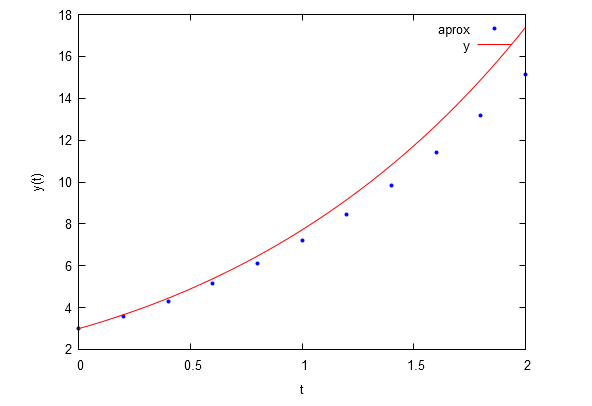
\includegraphics[width=10cm]{./Images/ejtp1-1.png}
				\caption{Aproximación a la solución con el método de Euler.}
			\end{figure}	
		\end{frame}		

		\begin{frame}{Ejercicio 1}
				\begin{table}[H]
					\centering
					\begin{tabular}{|| c | c | c | c | c||}
						\hline
						\hline $j$ &  $t_j $ & $y_j Explicito$ & $y_j Implicito$ & $y_j Euler$ \\
						\hline 0 & 0.0 & 3 & 3 & 3 \\
						\hline 1 & 0.2 & 3.656 & 3.66216 & 3.6 \\
						\hline 2 & 0.4 & 4.3952 & 4.453683 & 4.312 \\
						\hline 3 & 0.6 & 5.361014 & 5.385540 & 5.1424 \\
						\hline 4 & 0.8 & 6.433237 & 6.471135 & 6.09888 \\
						\hline 5 & 1.0 & 7.671749 & 7.726853 & 7.190656 \\
						\hline 6 & 1.2 & 9.095534 & 9.172720 & 8.428787 \\
						\hline 7 & 1.4 & 10.727752 & 10.833211 & 9.826544 \\
						\hline 8 & 1.6 & 12.596657 & 12.738239 & 11.399853 \\
						\hline 9 & 1.8 & 14.736722 & 14.924363 & 13.167824 \\
						\hline 10 & 2.0 & 17.190000 & 17.436269 & 15.153389 \\
						\hline
						\hline
					\end{tabular}
					\caption{Tabla comparativa con $h=0.2$}
				\end{table}	
		\end{frame}
		
		\begin{frame}{Ejercicio 1}
			\begin{figure}[h]
				\centering
				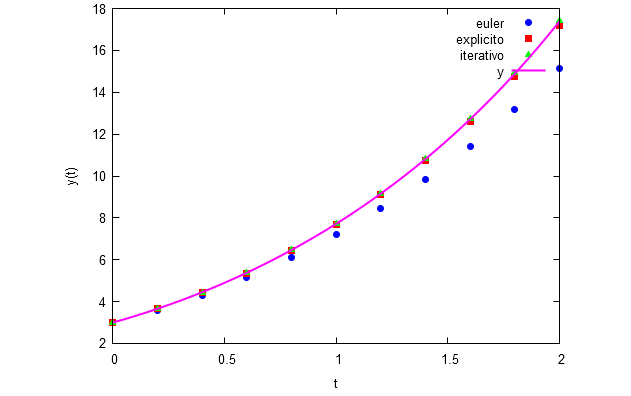
\includegraphics[width=10cm]{./Images/ejtp1-2.png}
				\caption{Aproximación a la solución con los métodos.}
			\end{figure}	
		\end{frame}
				
		\begin{frame}{Ejercicio 2}
			Dada la ecuación $y'=t+y^2$ con $y(1)=1$ aproximar mediante el método del trapecio: a) y(1,2) con 2 pasos (h=0,1) y b) y(1,2) con 4 pasos (h=0,05). Si el error global es de la forma $Ch^2$, estimar el valor de C a partir de los resultados anteriores. Determinar h para que el error sea del orden de $10^{-4}$.		
		\end{frame}
					
		\begin{frame}{Ejercicio 2}
			    \begin{table}[H]
			    	\centering
			    	\begin{tabular}{|| c | c | c | c | c ||}
			    		\hline
			    		\hline $j$ &  $t_{j-1}$ & $y_{j-1}$ & $t_j$ & $y_j$ \\
			    		\hline 1 & 1.00 & 2.000000 & 1.10 & 2.617500 \\
			    		\hline 2 & 1.10 & 2.617500 & 1.20 & 3.657368 \\
			    		\hline
			    		\hline
			    	\end{tabular}
			    	\caption{Trapecio con $h=0.1$}
			    \end{table}		
		\end{frame}
						
		\begin{frame}{Ejercicio 2}
				\begin{table}[H]
					\centering
				 	\begin{tabular}{|| c | c | c | c | c ||}
				 		\hline
				 		\hline $j$ &  $t_{j-1}$ & $y_{j-1}$ & $t_j$ & $y_j$ \\
				 		\hline 1 & 1.00 & 2.000000 & 1.05 & 2.277813 \\
				 		\hline 2 & 1.05 & 2.277813 & 1.10 & 2.628941 \\
				 		\hline 3 & 1.10 & 2.628941 & 1.15 & 3.087423 \\
				 		\hline 4 & 1.15 & 3.087423 & 1.20 & 3.712364 \\
				 		\hline
				 		\hline
				 	\end{tabular}
				 	\caption{Trapecio con $h=0.05$}
				 \end{table}						
		\end{frame}

		\begin{frame}{Ejercicio 2}
			\begin{itemize}
				\item $y(1.2) - 3.657368 = C(0.1)^2$.
				\item $y(1.2) - 3.712364 = C(0.05)^2$.
				\item Restando obtenemos que $C=7.33$.
				\item Para que sea de orden $10^{-4}$, el error debe ser $h=3.7$ $10^{-3}$
			\end{itemize}					
			
 
		\end{frame}
				
		\begin{frame}{Ejercicio 3}
			El movimiento de caída de un cuerpo de masa m en un medio que opone una resistencia proporcional al cuadrado de la velocidad está gobernado por la ecuación diferencial:
			
			\begin{equation}
			\frac{d^2s}{dt^2}=g-\frac{K}{m}(\frac{ds}{dt})^2
			\end{equation}
			
			siendo $g=10 \frac{m}{s^2}$ y $K \frac{kg}{s}$ una constante de proporcionalidad cuyo valor depende del problema concreto. Si el cuerpo se abandona sin velocidad inicial y las condiciones iniciales son
			
			
			\begin{equation}
			s(0)=s'(0)=0
			\end{equation}
			
			Calcular una tabla de valores de las funciones $s(t)$ y $s'(t)$ para dibujar sus gráficas en el intervalo $[0,1]$. Tomar $\frac{K}{m}=5$.
		\end{frame}
											
		\begin{frame}{Ejercicio 3}
			\begin{table}[H]
				\centering
				\begin{tabular}{|| c | c | c | c | c ||}
					\hline
					\hline $j$ &  $t_{j-1}$ & $(u_{j-1},v_{j-1})$ & $t_j$ & $(u_{j},v_{j})$ \\
					\hline 1 & 0.00 & 0.000000,0.000000 & 0.10 & 0.050000,0.750000 \\
					\hline 2 & 0.10 & 0.050000,0.750000 & 0.20 & 0.160938,1.070068 \\
					\hline 3 & 0.20 & 0.160938,1.070068 & 0.20 & 0.289318,1.223146 \\
					\hline 4 & 0.30 & 0.289318,1.223146 & 0.40 & 0.424231,1.305143 \\
					\hline 5 & 0.40 & 0.424231,1.305143 & 0.50 & 0.562160,1.351168 \\
					\hline 6 & 0.50 & 0.562160,1.351168 & 0.60 & 0.701635,1.377549 \\
					\hline 7 & 0.60 & 0.701635,1.377549 & 0.70 & 0.841949,1.392822 \\
					\hline 8 & 0.70 & 0.841949,1.392822 & 0.80 & 0.982733,1.401712 \\
					\hline 9 & 0.80 & 0.982733,1.401712 & 0.90 & 1.123784,1.406900 \\
					\hline 10 & 0.90 & 1.123784,1.406900 & 1.00 & 1.264990,1.409933 \\
					\hline
					\hline					
				\end{tabular}
				\caption{Trapecio para sistemas con $h=0.1$}
			\end{table}	
		\end{frame}
		
		\begin{frame}{Ejercicio 3}
			\begin{figure}[h]
				\centering
				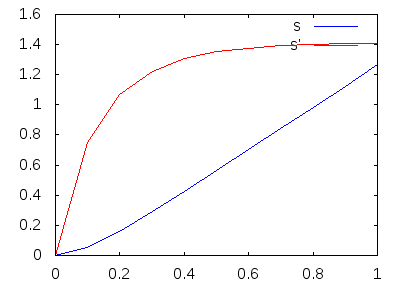
\includegraphics[width=10cm]{./Images/ejemplo3-1.png}
				\caption{Representación gráfica de s y s'.}
			\end{figure}	
		\end{frame}										
													
		\begin{frame}{Ejercicio 4: Algoritmo de Kahan para errores de redondeo}	

			\centering
			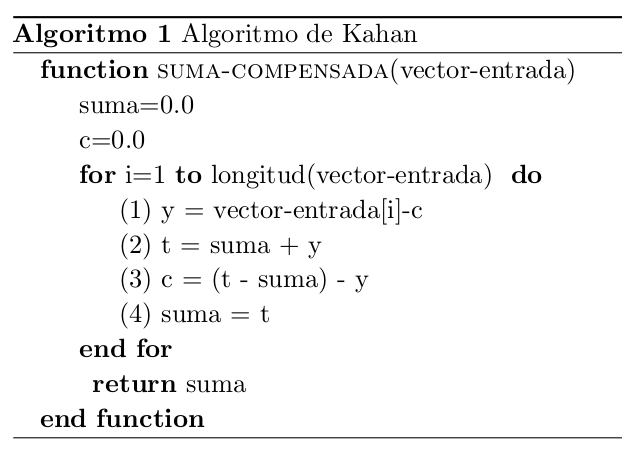
\includegraphics[width=0.8\textwidth]{./Images/kahan.png}
											
		\end{frame}	
		
		\begin{frame}{Ejercicio 4: Algoritmo de Kahan para errores de redondeo}	
			\fontsize{8}{10}\selectfont
			\begin{exercise}
				Supóngase que se utiliza aritmética decimal de seis dígitos, la suma actual es 10000.0 y los siguientes dos valores son 2.14159 y 2.71828. Comapre la suma usual con el algoritmo de Kahan.
			\end{exercise}
	
			\textbf{Método usual}
			\begin{itemize}
				\item Primera suma con redondeo: 10003.1 \\
				\item Segunda suma con redondeo: 10005.8 \\
			\end{itemize}
		
			\textbf{Método de Kahan}
			\begin{columns}
				\column{0.5\textwidth}
					\begin{itemize}
						\item Primera suma \\
						c = 0.0 \\
						y = 3.14159  \\
						t = 10000.0 + 3.14159 = 10003.14159 = 10003.1 \\
						c = (10003.1 - 10000.0) - 3.14159  = -.0415900 \\
						suma = 10003.1
					\end{itemize}										
				\column{0.5\textwidth}
					\begin{itemize}
						\item Segunda suma 	\\					
						y = 2.71828 - -.0.415900 = 2.75987 \\
						t = 10003.1 + 2.75987 = 10005.85987 = 10005.9 \\
						c = (10005.9 - 10003.1) - 2.75987 = .040130 \\
						suma = 10005.9 \\					
					\end{itemize}										
			\end{columns}
						
		\end{frame}									